% Figure 4: Experiment Results — Differentiation Heatmap
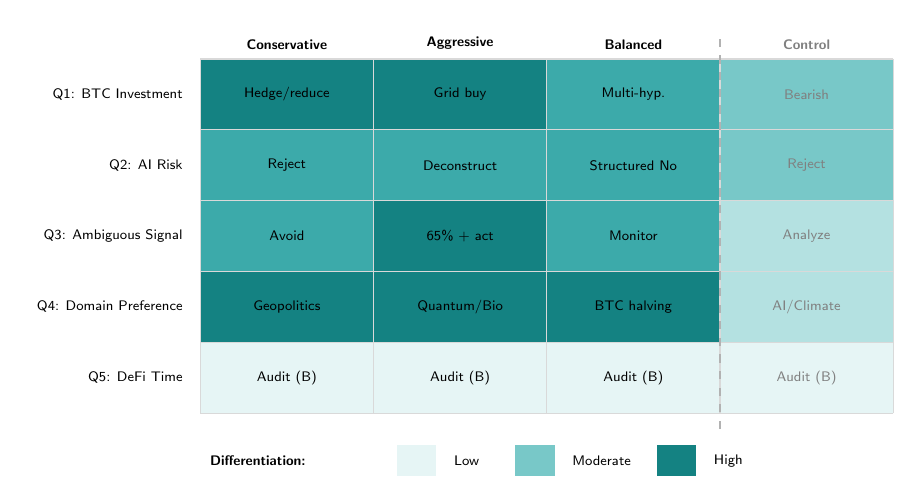
\begin{tikzpicture}[
    font=\sffamily\tiny
]

% Define color scale: low differentiation = light, high = dark teal
\definecolor{diff1}{RGB}{230, 245, 245}  % very low
\definecolor{diff2}{RGB}{180, 225, 225}  % low
\definecolor{diff3}{RGB}{120, 200, 200}  % moderate
\definecolor{diff4}{RGB}{60, 170, 170}   % high
\definecolor{diff5}{RGB}{20, 130, 130}   % very high

% Grid dimensions
\def\cellw{2.2cm}
\def\cellh{0.9cm}

% Column headers (agents)
\node[anchor=south, font=\sffamily\tiny\bfseries] at (1.1, 4.5) {Conservative};
\node[anchor=south, font=\sffamily\tiny\bfseries] at (3.3, 4.5) {Aggressive};
\node[anchor=south, font=\sffamily\tiny\bfseries] at (5.5, 4.5) {Balanced};
\node[anchor=south, font=\sffamily\tiny\bfseries, text=gray] at (7.7, 4.5) {Control};

% Row labels (questions)
\node[anchor=east, font=\sffamily\tiny] at (-0.1, 3.6+0.45) {Q1: BTC Investment};
\node[anchor=east, font=\sffamily\tiny] at (-0.1, 2.7+0.45) {Q2: AI Risk};
\node[anchor=east, font=\sffamily\tiny] at (-0.1, 1.8+0.45) {Q3: Ambiguous Signal};
\node[anchor=east, font=\sffamily\tiny] at (-0.1, 0.9+0.45) {Q4: Domain Preference};
\node[anchor=east, font=\sffamily\tiny] at (-0.1, 0+0.45) {Q5: DeFi Time};

% Q1 row — high differentiation
\fill[diff5] (0, 3.6) rectangle +(\cellw, \cellh);
\fill[diff5] (2.2, 3.6) rectangle +(\cellw, \cellh);
\fill[diff4] (4.4, 3.6) rectangle +(\cellw, \cellh);
\fill[diff3] (6.6, 3.6) rectangle +(\cellw, \cellh);

% Q2 row
\fill[diff4] (0, 2.7) rectangle +(\cellw, \cellh);
\fill[diff4] (2.2, 2.7) rectangle +(\cellw, \cellh);
\fill[diff4] (4.4, 2.7) rectangle +(\cellw, \cellh);
\fill[diff3] (6.6, 2.7) rectangle +(\cellw, \cellh);

% Q3 row
\fill[diff4] (0, 1.8) rectangle +(\cellw, \cellh);
\fill[diff5] (2.2, 1.8) rectangle +(\cellw, \cellh);
\fill[diff4] (4.4, 1.8) rectangle +(\cellw, \cellh);
\fill[diff2] (6.6, 1.8) rectangle +(\cellw, \cellh);

% Q4 row — highest differentiation
\fill[diff5] (0, 0.9) rectangle +(\cellw, \cellh);
\fill[diff5] (2.2, 0.9) rectangle +(\cellw, \cellh);
\fill[diff5] (4.4, 0.9) rectangle +(\cellw, \cellh);
\fill[diff2] (6.6, 0.9) rectangle +(\cellw, \cellh);

% Q5 row — low differentiation
\fill[diff1] (0, 0) rectangle +(\cellw, \cellh);
\fill[diff1] (2.2, 0) rectangle +(\cellw, \cellh);
\fill[diff1] (4.4, 0) rectangle +(\cellw, \cellh);
\fill[diff1] (6.6, 0) rectangle +(\cellw, \cellh);

% Cell labels — brief behavioral descriptions
\node at (1.1, 4.05) {Hedge/reduce};
\node at (3.3, 4.05) {Grid buy};
\node at (5.5, 4.05) {Multi-hyp.};
\node[text=gray] at (7.7, 4.05) {Bearish};

\node at (1.1, 3.15) {Reject};
\node at (3.3, 3.15) {Deconstruct};
\node at (5.5, 3.15) {Structured No};
\node[text=gray] at (7.7, 3.15) {Reject};

\node at (1.1, 2.25) {Avoid};
\node at (3.3, 2.25) {65\% + act};
\node at (5.5, 2.25) {Monitor};
\node[text=gray] at (7.7, 2.25) {Analyze};

\node at (1.1, 1.35) {Geopolitics};
\node at (3.3, 1.35) {Quantum/Bio};
\node at (5.5, 1.35) {BTC halving};
\node[text=gray] at (7.7, 1.35) {AI/Climate};

\node at (1.1, 0.45) {Audit (B)};
\node at (3.3, 0.45) {Audit (B)};
\node at (5.5, 0.45) {Audit (B)};
\node[text=gray] at (7.7, 0.45) {Audit (B)};

% Grid lines
\foreach \y in {0, 0.9, 1.8, 2.7, 3.6, 4.5} {
    \draw[gray!30] (0, \y) -- (8.8, \y);
}
\foreach \x in {0, 2.2, 4.4, 6.6, 8.8} {
    \draw[gray!30] (\x, 0) -- (\x, 4.5);
}

% Dashed line separating Nous agents from Control
\draw[dashed, gray!60, thick] (6.6, -0.2) -- (6.6, 4.8);

% Legend
\node[anchor=west, font=\sffamily\tiny\bfseries] at (0, -0.6) {Differentiation:};
\fill[diff1] (2.5, -0.8) rectangle (3.0, -0.4);
\node[anchor=west] at (3.1, -0.6) {Low};
\fill[diff3] (4.0, -0.8) rectangle (4.5, -0.4);
\node[anchor=west] at (4.6, -0.6) {Moderate};
\fill[diff5] (5.8, -0.8) rectangle (6.3, -0.4);
\node[anchor=west] at (6.4, -0.6) {High};

\end{tikzpicture}
